% CVPR 2022 Paper Template
% based on the CVPR template provided by Ming-Ming Cheng (https://github.com/MCG-NKU/CVPR_Template)
% modified and extended by Stefan Roth (stefan.roth@NOSPAMtu-darmstadt.de)

\documentclass[10pt,twocolumn,letterpaper]{article}

%%%%%%%%% PAPER TYPE  - PLEASE UPDATE FOR FINAL VERSION
% \usepackage[review]{cvpr}      % To produce the REVIEW version
\usepackage{cvpr}              % To produce the CAMERA-READY version
%\usepackage[pagenumbers]{cvpr} % To force page numbers, e.g. for an arXiv version

% Include other packages here, before hyperref.
\usepackage{graphicx}
\usepackage{amsmath}
\usepackage{amssymb}
\usepackage{booktabs}


% It is strongly recommended to use hyperref, especially for the review version.
% hyperref with option pagebackref eases the reviewers' job.
% Please disable hyperref *only* if you encounter grave issues, e.g. with the
% file validation for the camera-ready version.
%
% If you comment hyperref and then uncomment it, you should delete
% ReviewTempalte.aux before re-running LaTeX.
% (Or just hit 'q' on the first LaTeX run, let it finish, and you
%  should be clear).
\usepackage[pagebackref,breaklinks,colorlinks]{hyperref}


% Support for easy cross-referencing
\usepackage[capitalize]{cleveref}
\crefname{section}{Sec.}{Secs.}
\Crefname{section}{Section}{Sections}
\Crefname{table}{Table}{Tables}
\crefname{table}{Tab.}{Tabs.}


%%%%%%%%% PAPER ID  - PLEASE UPDATE
\def\cvprPaperID{*****} % *** Enter the CVPR Paper ID here
\def\confName{CVPR}
\def\confYear{2022}


\begin{document}

%%%%%%%%% TITLE - PLEASE UPDATE
\title{Project Milestone for Text Eraser on Image}

\author{
Leung Tsz Kit Gary\\
{\tt\small tkleungal@connect.ust.hk}
% For a paper whose authors are all at the same institution,
% omit the following lines up until the closing ``}''.
% Additional authors and addresses can be added with ``\and'',
% just like the second author.
% To save space, use either the email address or home page, not both
\and
Ip Marisa\\
{\tt\small mip@connect.ust.hk}
}
\maketitle

%%%%%%%%% ABSTRACT
\begin{abstract}
    In this project, we aim to develop a model solution to perform the task of text removal on images.
    A mixed deep learning solution, with the use of image text segmentation and inpainting models, will be proposed to achieve this task.
    Various changes have been made to both models' architectures to improve their performance, including the increase of depth on the pathways
    and the introduction of a rule-based mask-awareness mechanism. The model results are visualized and evaluated, with a visible improvement 
    in the performance of the models compared to their corresponding baseline models. 
    A pipeline has also been created to combine the 2 models together for prediction, performing the task of text removal on images.
    The project repository can be accessed with cloning the following \href{https://github.com/GLGDLY/ELEC4240_project}{Github link}.
\end{abstract}

%%%%%%%%% BODY TEXT
\section{Introduction}
\label{sec:intro}

In this project, we aim to develop a model solution to perform the task of text removal on images. 
The idea was initiated from the problem that most of the text eraser solutions online currently are performed with English word processing, 
with bad performance on the processing of Chinese characters mixed with English characters. 
However, in the Hong Kong environment, such a case is a common scenario. Therefore, we would like to develop a solution that can handle such use case.

To approach the problem, a mixed deep learning solution will be proposed, with the following 2 parts:

\begin{enumerate}
  \item Image text segmentation
  \item Inpainting
\end{enumerate}

For the flow of the solution, an image text segmentation network will first be computed with the input image.
The output of the segmentation will then be a mask of the target text region which can then be used as one of the input of the 
inpainting model to remove the text region from the image, resulting in the final output image with the text removed. The 
project repository can be accessed with cloning the following \href{https://github.com/GLGDLY/ELEC4240_project}{Github link}.

\section{Related Work}
\label{sec:related_work}

\subsection{Image text segmentation}

\subsection{Inpainting}

Inpainting is a well-studied problem in computer vision, with various approaches proposed to fill in missing or corrupted regions of images.
The following are some of the most notable works that this project has been inspired by:

\begin{itemize}
    \item \textbf{Pix2Pix}~\cite{Isola2018}: This approach uses a conditional Generative Adversarial Network (cGAN) to learn the mapping between input and output images. 
    The generator is a U-Net architecture, while the discriminator is a PatchGAN model. This method has been widely used for image-to-image translation tasks, including inpainting.
    However, for inpainting tasks, it does not explicitly consider the masked regions, which can lead to artifacts in the generated images, for examle, when the input image is having a 
    white background or when zero paddings are performed in the edge cases.
    \item \textbf{Partial Convolution}~\cite{Liu2018}: This approach introduces a partial convolution layer that only considers valid pixels in the input image, 
    effectively ignoring the masked regions. This allows the model to learn features from the surrounding context while avoiding artifacts in the inpainted region.
    However, this work only proposed a single convolution layer, with an example of using VGG16 as the backbone of the model.
\end{itemize}

The above works have inspired the design of our inpainting model, where we aim to combine the strengths of both approaches.

\section{Problem statement}

\subsection{Image text segmentation}
To commence with, the first problem of this project is to develop an image text segmentation model capable of detecting and segmenting text regions from images. 
The model is expected to produce a mask for the inpainting process to work with, where text regions are marked as 1 and non-text regions are marked as 0 in the binary mask output.

To achieve this, the RCTW-17 dataset was used for providing pre-annotated images containing multi-language text in different styles and complex backgrounds.
A total of 12,263 images were selected, with 8,034 and 4,229 images in the training and testing dataset respectively. 
We will be working on another dataset shortly given the small dataset size RCTW is providing currently. The current dataset can be accessed with the following 
\href{https://drive.google.com/drive/folders/1BbLe23KN1At6xsItvBcj9dXhPv6LdQH_?usp=sharing}{Google Drive link}.

Making use with the above dataset, the bounding box annotations of the text regions provided were being processed and converted into binary mask images.
These image files are thus loaded as single-channel masks alongside their corresponding input images during the training process. 
It aims to provide accurate text region annotations, with their relative efficiency and impact on model performance to be analyzed in subsequent sections of this report. 
These binary masks serve dual purposes: they act as ground truth labels for training the segmentation model, and later provide a standardized format for the inpainting stage of the text removal pipeline.

It is expected that the model will be able to identify text regions across different languages, styles, and challenging image conditions. 
The resulting binary masks will serve as crucial input for the subsequent inpainting process, ensuring reliable text removal from images. 
The model's performance will be evaluated through multiple metrics tracked via TensorBoard:
\begin{enumerate}
    \item $IoU$: Intersection of Union of the predicted mask and the ground truth mask, should be maximized to ensure accurate localization
    \item $F1\;score$: The harmonic mean of precision and recall, should be maximized to achieve balance for accuracy 
    \item $Dice Loss$: To measure the overlap between predicted segmentation and ground truth masks, should be minimized for a better match
\end{enumerate}

\subsection{Inpainting}

The second problem of this project is to develop an inpainting model that can erase the text region from the image, given the mask of the text region by 
the image text segmentation model. The inpainting model will be trained with the input of the original image multiplied by the mask of the text region and 
the mask of the text region itself, while the output will be the final image with the text region removed.

With this objective, the COCO-Text dataset was selected, with filtering the images that contain no text into our training dataset. This dataset was 
chosen since it contains text labels that can be used to easily filter out images that contain or do not contain text, and thus can be used to build our training 
dataset that prevents our model from learning the wrong information like English text. With this approach, a total of 30,201 images were being selected, and with 
performing train-test split with a ratio of 0.8, the training dataset is having 24,160 images and the testing dataset is having 6,041 images currently. It is believed
that this dataset size may not be enough for the training of the inpainting model, but it can be used as a starting point for the development of the model for testing
the feasibility and performance for different model structures, and further data collection can be performed in the later stage of the project. The current dataset can
be accessed with the following 
\href{https://hkustconnect-my.sharepoint.com/:u:/g/personal/tkleungal_connect_ust_hk/EUJ-38d8cptNgW2RK0JzHI4BfIi5mXwbIEFObTG7ji9f8g?e=LqJ1Eu}{OneDrive link}.

With the above dataset as the ground truth, the model input is generated by multiplying the original image with an input mask, where 2 different approaches have been 
proposed and implemented. The first approach that we have tried is dynamically generating the mask of the ground truth image during the training process, with implementing
the mask generation as the loading process of the dataset. The second approach that we have tried is to pre-generate the mask of the ground truth image and save it as an image
file, then loading the image file to become a 1-channel mask when loading the ground truth image. The comparison of the 2 approaches will be discussed in the later 
section of this report.

The model is expected to achieve a realistic inpainting result with the text being erased, and the performance of the model is expected to be evaluated with the
use of TensorBoard. Considering a GAN-based model architecture, the evaluation of the model performance will be expected to be evaluated with the below metrics:
\begin{enumerate}
    \item $gen\_gan\_loss$: The loss of the generator in the GAN model, where for a generator that can better fool the discriminator, this loss should be minimized
    \item $gen\_l1\_loss$: Mean absolute error between the generated image and the ground truth, should be minimized to achieve a closer result to the ground truth
\end{enumerate}

The $gen\_total\_loss$ will then be a combination of the above 2 losses, with $LAMBDA$ as the weight of the $gen\_l1\_loss$ in the total loss calculation. The $LAMBDA$
value is currently set as 100, while further testing will be performed to find the optimal value for the $LAMBDA$, or evaluate the performance when using a dynamically
changing $LAMBDA$ value during the training process.

\section{Methodology}

\subsection{Image text segmentation}

In accordance with the aforementioned problem statement, an improved architecture was proposed and designed on the basis of the U-Net model. 
The original U-Net architecture is of encoder-decoder form with the encoder slowly reducing the spatial dimensions of the input image with 
deeper feature representation being learned and the decoder generating the segmentation map by upsampling the said features. 
In addition with the skip connections, which is to preserve spatial information across different scales, can make the model to be suitable
for precise segmentation tasks. Nevertheless, since the U-Net was originally designed for biomedical image segmentation, 
some modifications are needed in order to fit the challenging nature of mixed-language text segmentation where text features 
vary extensively in terms of style, size, and orientation.

To enhance its performance even more, various modifications are proposed to be applied. Firstly, the encoder pathway will be enhanced through replacing 
the vanilla convolutional blocks with ResNet blocks. With this modification, the model has the capability of learning abstract-level features 
by exploiting skip connections of the ResNet block architecture for alleviating the vanishing gradient issue and deep feature extraction. 
Secondly, an attention mechanism will be introduced in skip connections across decoder and encoder paths. Unlike the original direct skip connections, 
the attention gates allow the model to focus on meaningful areas of text and disregard background noise, 
achieved as: $F_{att} = \sigma(W_x * x + W_g * g + b)$, where $x$ represents features from the encoder path and $g$ is the gated signal from the decoder path. 
Lastly, the decoder path will be reinforced further with additional convolutional layers to better restore fine text detail. 
By increasing the depth of the decoder further, we are confident that the model can recover intricate text region structures better, 
which will result in more accurate segmentation output.

With these architectural changes, the model shows improved text segmentation capability. However, there still exists a problem 
in processing text with extreme size or extreme deformation. To avoid this, we are using a multi-scale training strategy where the model is trained 
to learn scale-invariant features by feeding input images at various resolutions. In addition, to further enhance the capability of the model 
to distinguish text from text-like patterns in complex backgrounds, a dual-attention mechanism is suggested for both spatial and channel-wise operations. 
The purpose of the spatial attention is to locate the text areas, and channel attention is applied to the feature channels best fit for the nature of the text. 
These mechanisms are computed as: $A_s = \sigma(Conv(Concat[AvgPool(F); MaxPool(F)]))$ for spatial attention and $A_c = \sigma(MLP(AvgPool(F)))$ 
for channel attention, with F being the input feature maps. The efficiency of these different architectural blocks will be contrasted 
in detail in the rest of this report, with future potential exploration of hybrid solutions combining different attention mechanisms.

\subsection{Inpainting}

With the above problem statement, an architecture modified from the pix2pix architecture by Isola~\etal\cite{Isola2018} was proposed and implemented. The generator of the pix2pix architecture is
a U-Net model with skip connections to preserve spatial and high-level details of the input image for the inpainting model, while the discriminator is a PatchGAN
model with Binary Cross Entropy loss. However, this architecture was initiated by its authors as a solution to the image-to-image translation task, mapping the input image to the output image 
with learning the whole input image features and generating a full output image. This does not fully match our requirements, where we would like our model to learn the features of the input images, 
while only focus on generating the filling of the masked region. Therefore, several modifications would be needed to the generator of the pix2pix architecture for, firstly, prevent the model from updating
the non-masked region of the input image, and second, only apply gradient updates to the masked region regarding the loss calculation on the output image. These were then implemented by modifying 
the output of the generator by multiplying the output with the mask together with a direct mapping of the non-masked region of the input to the output. For the loss calculation, the L1 loss was 
also needed to be modified for only consider the masked region of the output. This was implemented by the following: $l1\_loss = reduce\_mean(\mid(target - gen\_output) \times (1 - mask)\mid)$, 
where the mean absolute error was calculated only on the masked region of the output image.

With the above modifications to the pix2pix architecture, the model can now be correctly trained and generate an output image with the masked region being inpainted. However, as the model now 
consider the masked region also as valid input, but only handling the mask on the final output, with the fact that we are multiplying the original image with the mask to generate the input image, 
the model need extra learning steps to learn to use the surrounding information of the masked region but not the masked region itself, leading to potentially slower convergence of the model. Also,
as the model do not have the mask information, as well as the awareness of the masked region, it might be treating every pure white region as the masked region, putting wrong attention to the 
non-masked white region, or putting incorrect attention to the padding region on the edge of the input image. As a result, there is a need to introduce a mask-awareness mechanism to the 
model, forcing the model to ignore the correct masked region and only use the non-masked region as valid features to generate the output. This was implemented by introducing the Nvidia's 
Partial Convolution approach~\cite{Liu2018}, which provides a rule-based special awareness mechanism to emphasize the convolution of the model learning on the non-masked region. The final 
generator architecture was then implemented with 2 main possibilities, with fully using standard convolution layers, and with fully using partial convolution layers. The performance of these 2 
different generator architectures will be evaluated in the later section of this report, while investigation on a mixed approach was also performed but deprecated due to the fact that these 2 layers 
might destroy the feature maps of each other, leading to a worse performance on places like the edge of the image than the pure partial convolution approach.

The discriminator is the PatchGAN model from the pix2pix architecture with Binary Cross Entropy loss. While a factor of $LAMBDA$ is used to balance the generator loss and the discriminator loss as in 
\cref{eq:inpainting_loss}, various values of this $LAMBDA$ value would be tested to find the optimal value for our use case. The depth of the discriminator was also considered and modified to try 
improve the performance.  

\begin{equation}
    L_{total} = L_{gen\_gan} + LAMBDA \times L_{gen\_l1}
    \label{eq:inpainting_loss}
\end{equation}

\section{Experiments}

\subsection{Image text segmentation}
Initial tests were conducted to evaluate the performance of different architectural approaches in the segmentation model, maintaining consistent 
hyperparameters and training epochs across experiments. The primary focus at this stage is on the Dice Loss and IoU metrics, as these 
directly reflect the model's ability to accurately identify text regions. 

Firstly, the baseline U-Net occasionally produces fragmented text regions and struggles with text at varying scales, particularly with Chinese characters 
with different text scales and styles. This model therefore aims to learn distinguish text from background, where the skip connections with attention gates 
and residual blocks might help improve gradient flow and maintain precise text boundaries. Currently, the implemented model provided the crucial first step 
of identifying text regions that need to be inpainted by outputting the binary masks, with conducting data processing to generate image mask layers for the 
RCTW-dataset (as shown in \cref{fig:verify}).

\begin{figure}[t]
    \centering
    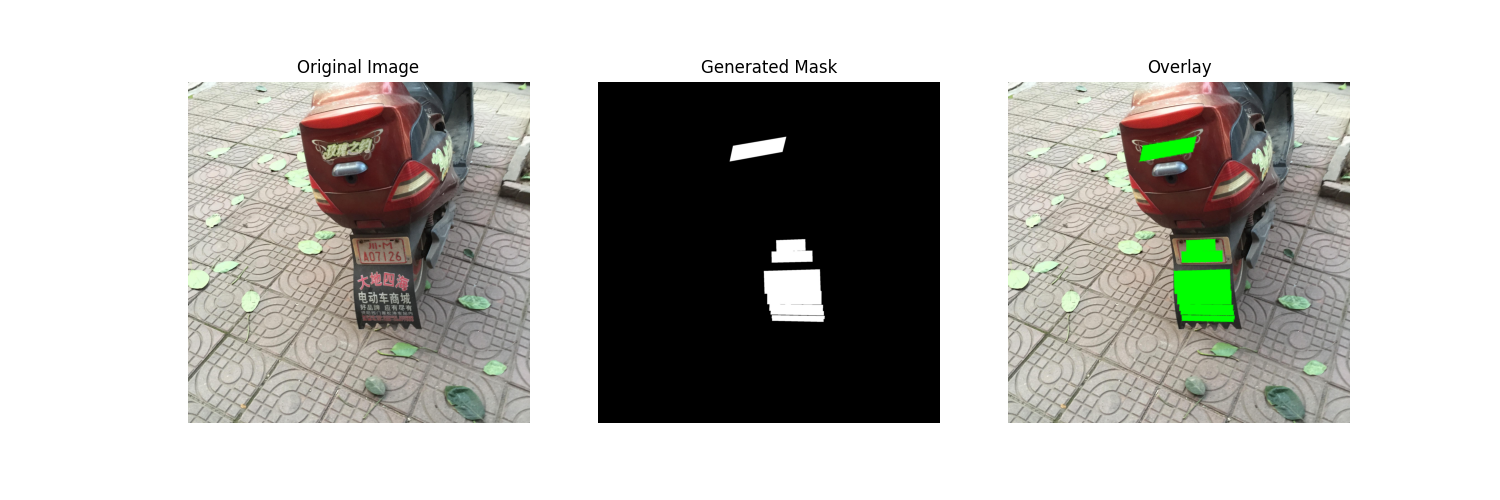
\includegraphics[width=\linewidth]{figures/milestone/verify_1.png}
    \caption{Example of mask image generated with the RCTW-dataset.}
    \label{fig:verify}
\end{figure}

% Firstly, the enhanced architecture is illustrated in \cref{fig:model1}. The baseline U-Net occasionally produces fragmented text regions and 
% struggles with text at varying scales, particularly with Chinese characters with different text scales and styles. The model learns to distinguish text 
% from background, where the skip connections help maintain precise text boundaries. This model provided the crucial first step of identifying text regions 
% that need to be inpainted by outputting the binary masks. 

% \begin{figure}[t]
%     \centering
%     \includegraphics[scale=0.01]{figures/milestone/model.png}
%     \caption{Output architectural image of the model.}
%     \label{fig:model1}
% \end{figure}

Secondly, the evaluation metrics from the training process demonstrate progress in the model's ability to segment text regions. 
As shown in \cref{fig:out_iou} and \cref{fig:out_loss}, the IoU metric generally increases over 4,000 iterations, while the loss function correspondingly decreases. 
Since the IoU metric directly measures the overlap between predicted and actual text regions, a higher IoU indicates more precise text localization, 
which is critical for subsequent inpainting tasks. The loss function, on the other hand, reflects the model's learning process, with a decreasing trend indicating improved performance.
The current results, with overall a positive trajectory of IoU and decreasing trend on the loss, show the model's ability to effectively learn and adapt to the dataset, distinguishing 
text regions across our diverse bilingual dataset, yet the model is still in the early stages of convergence. In subsequent stages, we will focus on evaluating and improving the model's 
performance through different hyperparameters and architectural modifications, including the introduction of attention mechanisms and  modifications to the encoder pathway, as 
mentioned in the previous sections.

\begin{figure}[t]
    \centering
    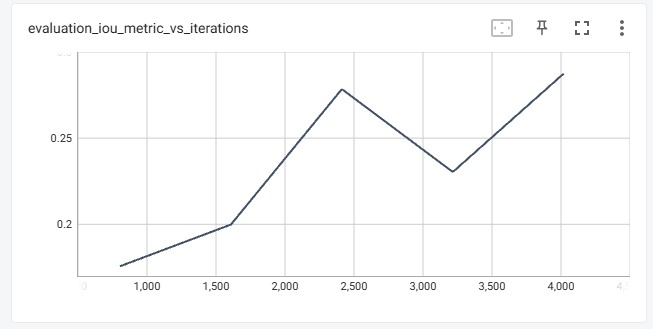
\includegraphics[width=\linewidth]{figures/milestone/out_iou.jpg}
    \caption{Output image of the IoU metrics with respect to the number of iterations. }
    \label{fig:out_iou}
\end{figure}

\begin{figure}[t]
    \centering
    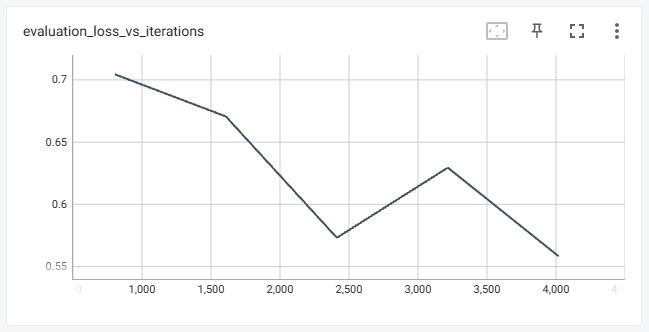
\includegraphics[width=\linewidth]{figures/milestone/out_loss.jpg}
    \caption{Output image of the dice loss with respect to the number of iterations. }
    \label{fig:out_loss}
\end{figure}

\subsection{Inpainting}

With the dataset structure and architecture mentioned above, tests were performed to evaluate the performance of different approaches, where same parameters and epochs were applied to these 
approaches. As we are mainly evaluating the generator currently with the use of $LAMBDA = 100$ in the total generator loss calculation, where the discriminator is not yet significant and will be
evaluated in the later stage of the project, we will mainly focus on the $gen\_l1\_loss$ for evaluation in this stage. 

First, considering the mask generation approach, both of the approaches were tested and the results were compared as shown in \cref{fig:gen_vs_fix}. It is obvious that the dynamically generated mask 
approach is converging slower than the fixed mask approach. This is as expected, as the dynamically generated mask approach is generating the mask during the training process, leading to extra learning
steps for the model to learn the mask information. Therefore, in the current stage, to increase the development and iteration speed of our model, the fixed mask approach would be selected for now.

\begin{figure}[t]
    \centering
    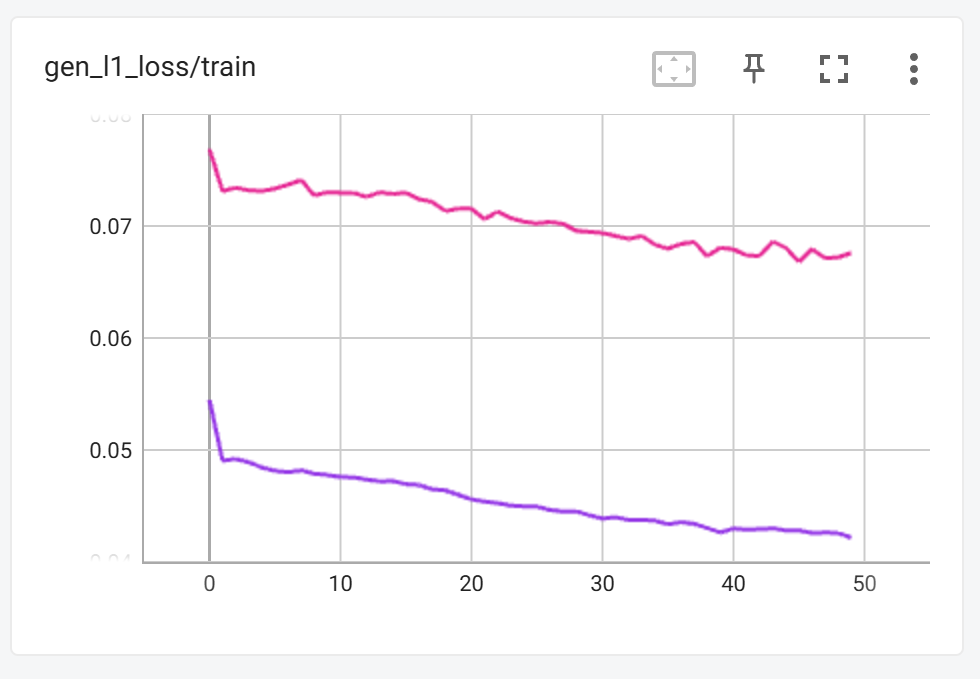
\includegraphics[width=\linewidth]{figures/milestone/gen_vs_fix.png}
    \caption{Comparison of the training $gen\_l1\_loss$, with pink line as the dynamically generated mask approach, and purple line as the fixed mask approach.}
    \label{fig:gen_vs_fix}
\end{figure}

Second, considering the generator architecture, the standard convolution approach and the partial convolution approach were tested and the results were compared as shown in \cref{fig:stand_vs_pconv}. It is 
clear that the partial convolution has a much better convergence speed than the standard convolution approach, proving the idea of using the partial convolution layers to provide the mask-awareness towards 
the generator. This can also be shown from the outputs (\cref{fig:out_standconv} and \cref{fig:out_pconv}) of the 2 different approaches, where it can be seen that the standard convolution approach is 
generating the masked region with an incoherent boundary, while the partial convolution approach has a better performance on reducing seams. The texture of the output image is also more realistic with the 
partial convolution approach, in which we can see the standard convolution approach is generating point-like textures on the masked region as a result of invalid "0" values are also being learned by the model. 
With such observation, the partial convolution approach would be preferable for the further development of the model. 

\begin{figure}[t]
    \centering
    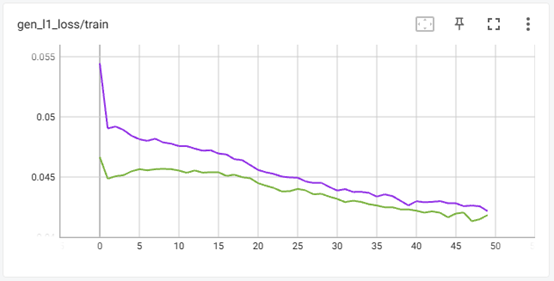
\includegraphics[width=\linewidth]{figures/milestone/stand_vs_pconv.png}
    \caption{Comparison of the training $gen\_l1\_loss$, with purple line as the standard convolution approach, and green line as the partial convolution approach.}
    \label{fig:stand_vs_pconv}
\end{figure}

\begin{figure}[t]
    \centering
    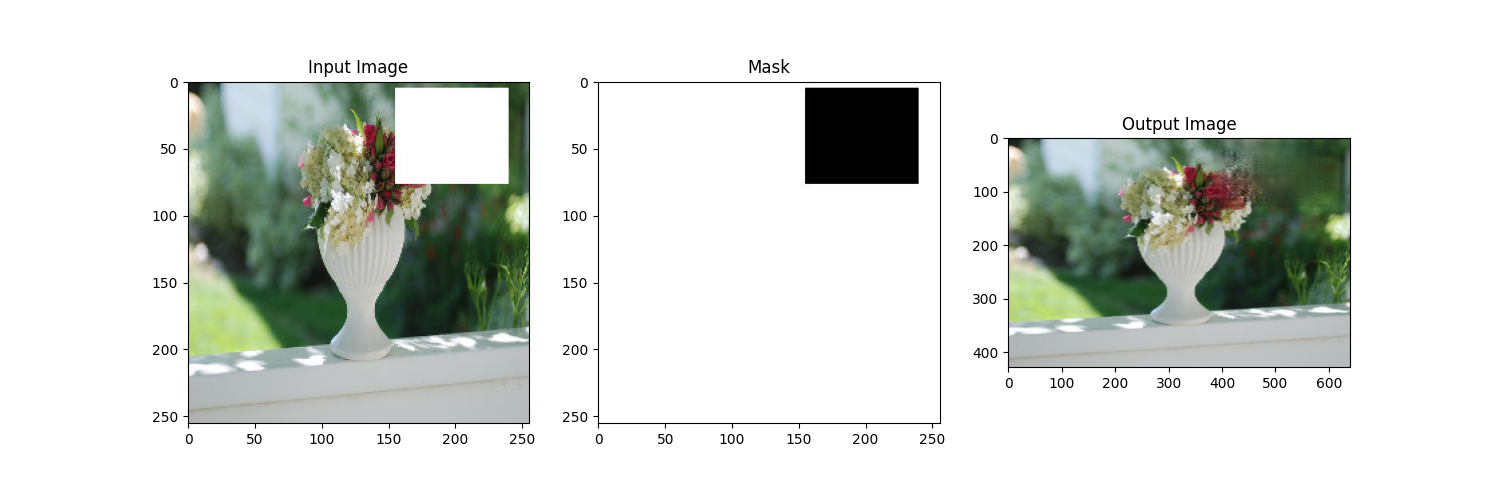
\includegraphics[width=\linewidth]{figures/milestone/out_standconv.png}
    \caption{Output image of the standard convolution approach.}
    \label{fig:out_standconv}
\end{figure}

\begin{figure}[t]
    \centering
    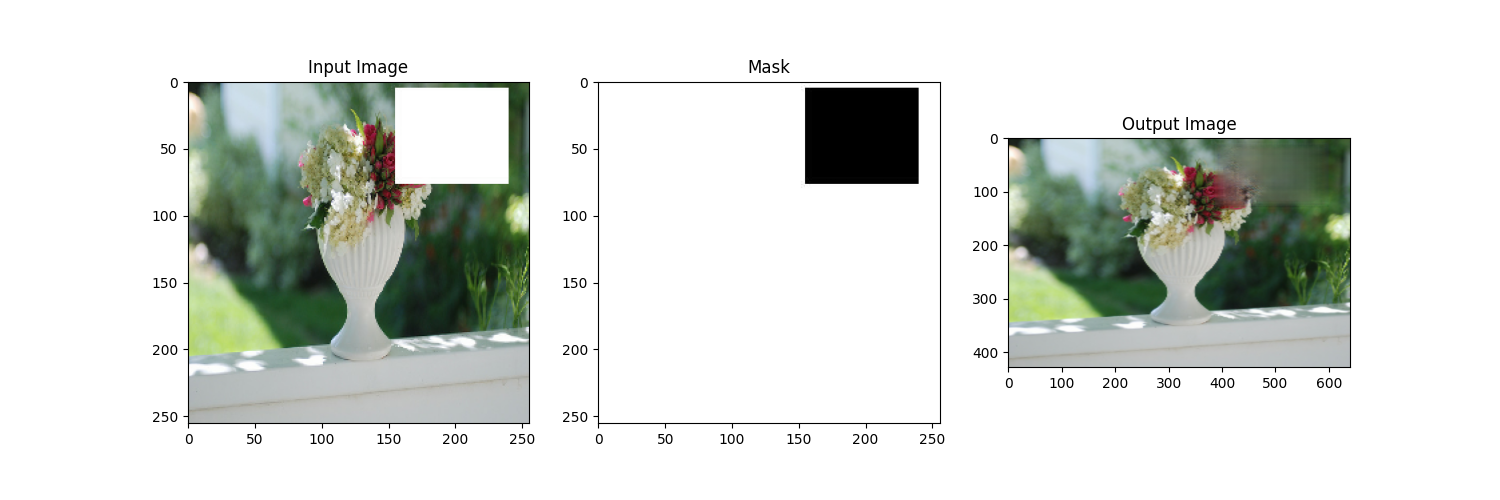
\includegraphics[width=\linewidth]{figures/milestone/out_pconv.png}
    \caption{Output image of the partial convolution approach.}
    \label{fig:out_pconv}
\end{figure}

On the other hand, Various values of $LAMBDA$ were also tested to find the optimal value for our use case. As shown in \cref{fig:lambda}, $LAMBDA = 50$ shows a relatively balanced performance on 
the generator l1 loss, which represents the mean absolute error between the generated image and the ground truth, and the generator gan loss, which represents the loss of the generator in the GAN model.
The $LAMBDA = 10$ shows a much unstable performance on the generator l1 loss, which is not ideal for the model to learn the features of the input image. The $LAMBDA = 100$ shows a similar performance to the
$LAMBDA = 50$, but the value indicates that the loss function is giving less weight to the discriminator result. As a result, to keep a balance between the actual image and the discriminator, the $LAMBDA = 50$ 
would be selected for the further development of the model.

\begin{figure}[t]
    \centering
    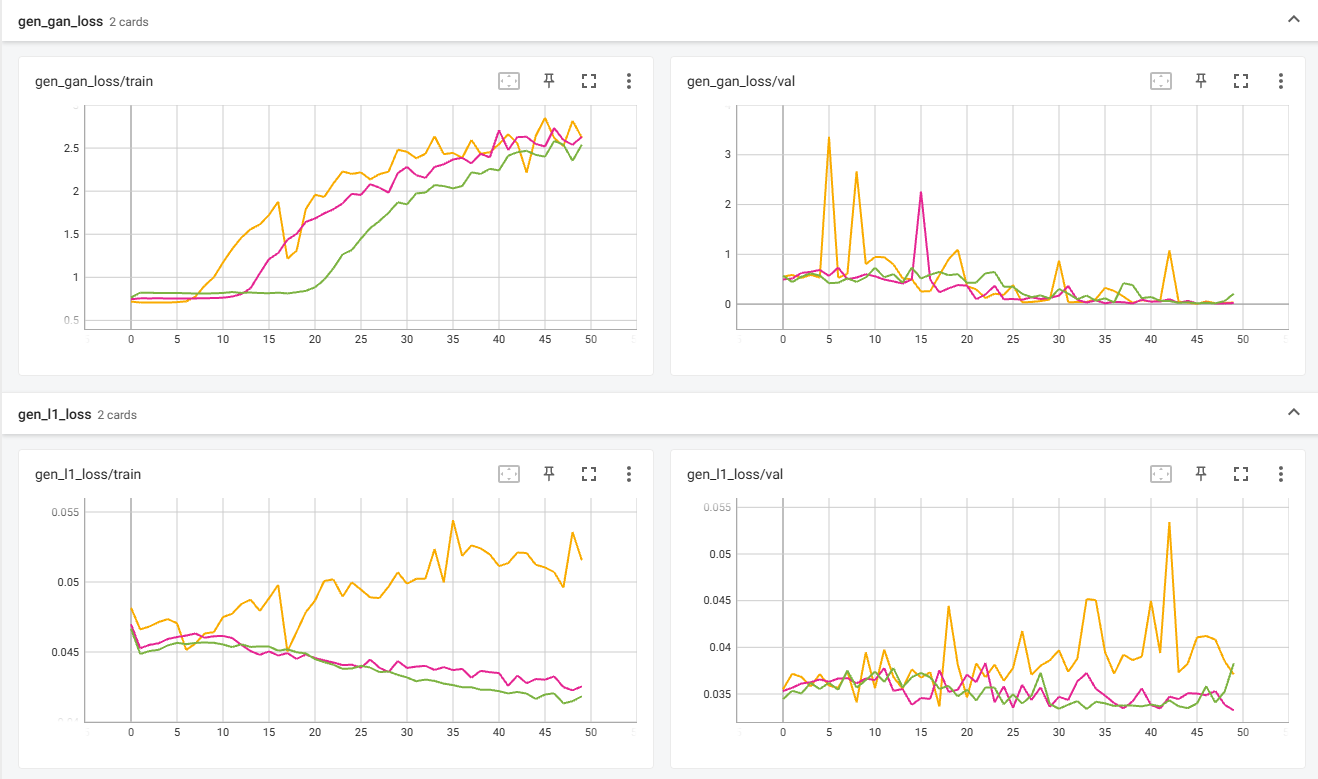
\includegraphics[width=\linewidth]{figures/milestone/lambda.png}
    \caption{Comparison of the training $gen\_l1\_loss$, with orange line as the $LAMBDA = 10$, purple-red line as the $LAMBDA = 50$, green line as the $LAMBDA = 100$.}
    \label{fig:lambda}
\end{figure}

However, from the above experiments, it can be seen that the discriminator is clearly overfitting during the training process, which might over-penalize the generator and lead to a worse performance of the 
generator. As a result, 

\section{Conclusion}

This project has devdeloped an mixed model pipeline to perform the task of text removal on images. By utilizing both of the image text segmentation and inpainting models,
the model is able to generate a mask of the text region and then inpaint the text region with the surrounding information. An example can be shown in \cref{fig:final_result},
showing a successful removal of the text region from the input image.

%%%% TODO: add the final result image
% \begin{figure}[t]
%     \centering
%     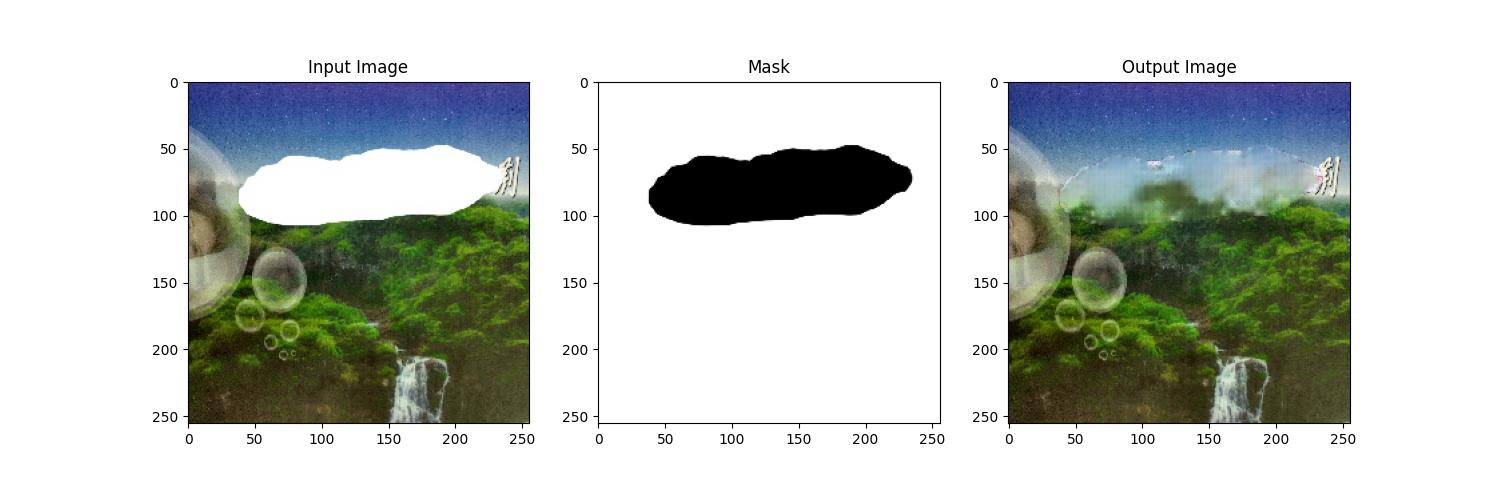
\includegraphics[width=\linewidth]{figures/milestone/final_result.png}
%     \caption{Example of the final result of the pipeline.}
%     \label{fig:final_result}
% \end{figure}

From this project, we have built concrete experiences on the development of deep learning models, with the understanding towards not only the model training and evaluation process, but also the 
data processing and the improvements of the model architecture. The project has also provided us with the opportunity to explore the different model architectures and the different approaches to 
improve the performance of the model, with the understanding of the advantages and disadvantages of each approach. For example, the understanding towards why the partial convolution approach is
better than the standard convolution approach has noticed us on the potential drawbacks of the zero padding on the standard convolution approach, and how rule-based special awareness mechanism can help
models to focus on specific regions of a image.

For the future work, the segmentation model can be further improved by exploring the use of different attention mechanisms, while the inpainting model can be further improved by exploring the use of 
diffusion models with a larger dataset. While this project can be further extended to specific applications like homework answer removal for primary school students to help them better review their homework
before exam, or with applications in the field of video editing, where the model can be used to remove unwanted text or objects from videos.

\section{Supplementary Material}

\begin{itemize}
    \item \textbf{Project repository}: The project repository can be accessed with the following \href{https://github.com/GLGDLY/ELEC4240_project}{hyperlink}
\end{itemize}

%%%%%%%%% REFERENCES
{\small
\bibliographystyle{ieee_fullname}
\bibliography{egbib_milestone}
}

\end{document}
